\documentclass[addpoints]{exam}
\usepackage[utf8]{inputenc}
\usepackage[portuguese]{babel}
\usepackage[LGRgreek]{mathastext}
\usepackage{graphicx,graphics}
\usepackage{hyperref}

\footer{}{\thepage}{}
 
\pointpoints{ponto}{pontos}
\bonuspointpoints{ponto extra}{pontos extra}
 
\totalformat{Pregunta \thequestion: \totalpoints pontos}
 
\chqword{Pregunta}
\chpgword{Página}
\chpword{Pontos}
\chbpword{Pontos extra}
\chsword{Pontos obtidos}
\chtword{Total}

\hqword{Questão}
\hpgword{Página}
\hpword{Pontos}
\hsword{Pontos obtidos}
\htword{Total}

 
\begin{document}
 
\begin{center}
Eletrônica Básica II – EE640 U - Lista SPICE 1
\end{center}
 
\vspace{5mm}
 
\makebox[0.72\textwidth]{Nome: \enspace\hrulefill}
\hfill
\makebox[0.2\textwidth]{RA: \enspace\hrulefill}

\begin{center}
A lista deve ser entregue até dia \textbf{01-01-1968}

\vspace{5mm}

Use o seu RA como \textit{\textbf{abcdef}}, exemplo: para 123456, ab=12, ef=56 e assim port diante.

Utilize 0 como 10, 00 como 100. RA = 002220, ab=100, f=10
\end{center}

\hspace{2mm}

\begin{center}
\gradetable[h][questions]
\end{center}

\hspace{2mm}

\begin{questions}

\question Usando o modelo de pequenos sinais de um amplificador do circuito da Figura com o ganho A = 100+\textit{\textbf{de}}, C1 = 50+\textit{\textbf{f}} e C2 = 20+\textit{\textbf{c}}, apresente:

\begin{parts}
\part[2] As curvas de módulo e fase da resposta em frequência do circuito de 1 Hz a 1 GHz;
\part[2] Os valores das frequências de corte (pólos) e o valor da fase para essas frequências.
\end{parts}

\begin{center}
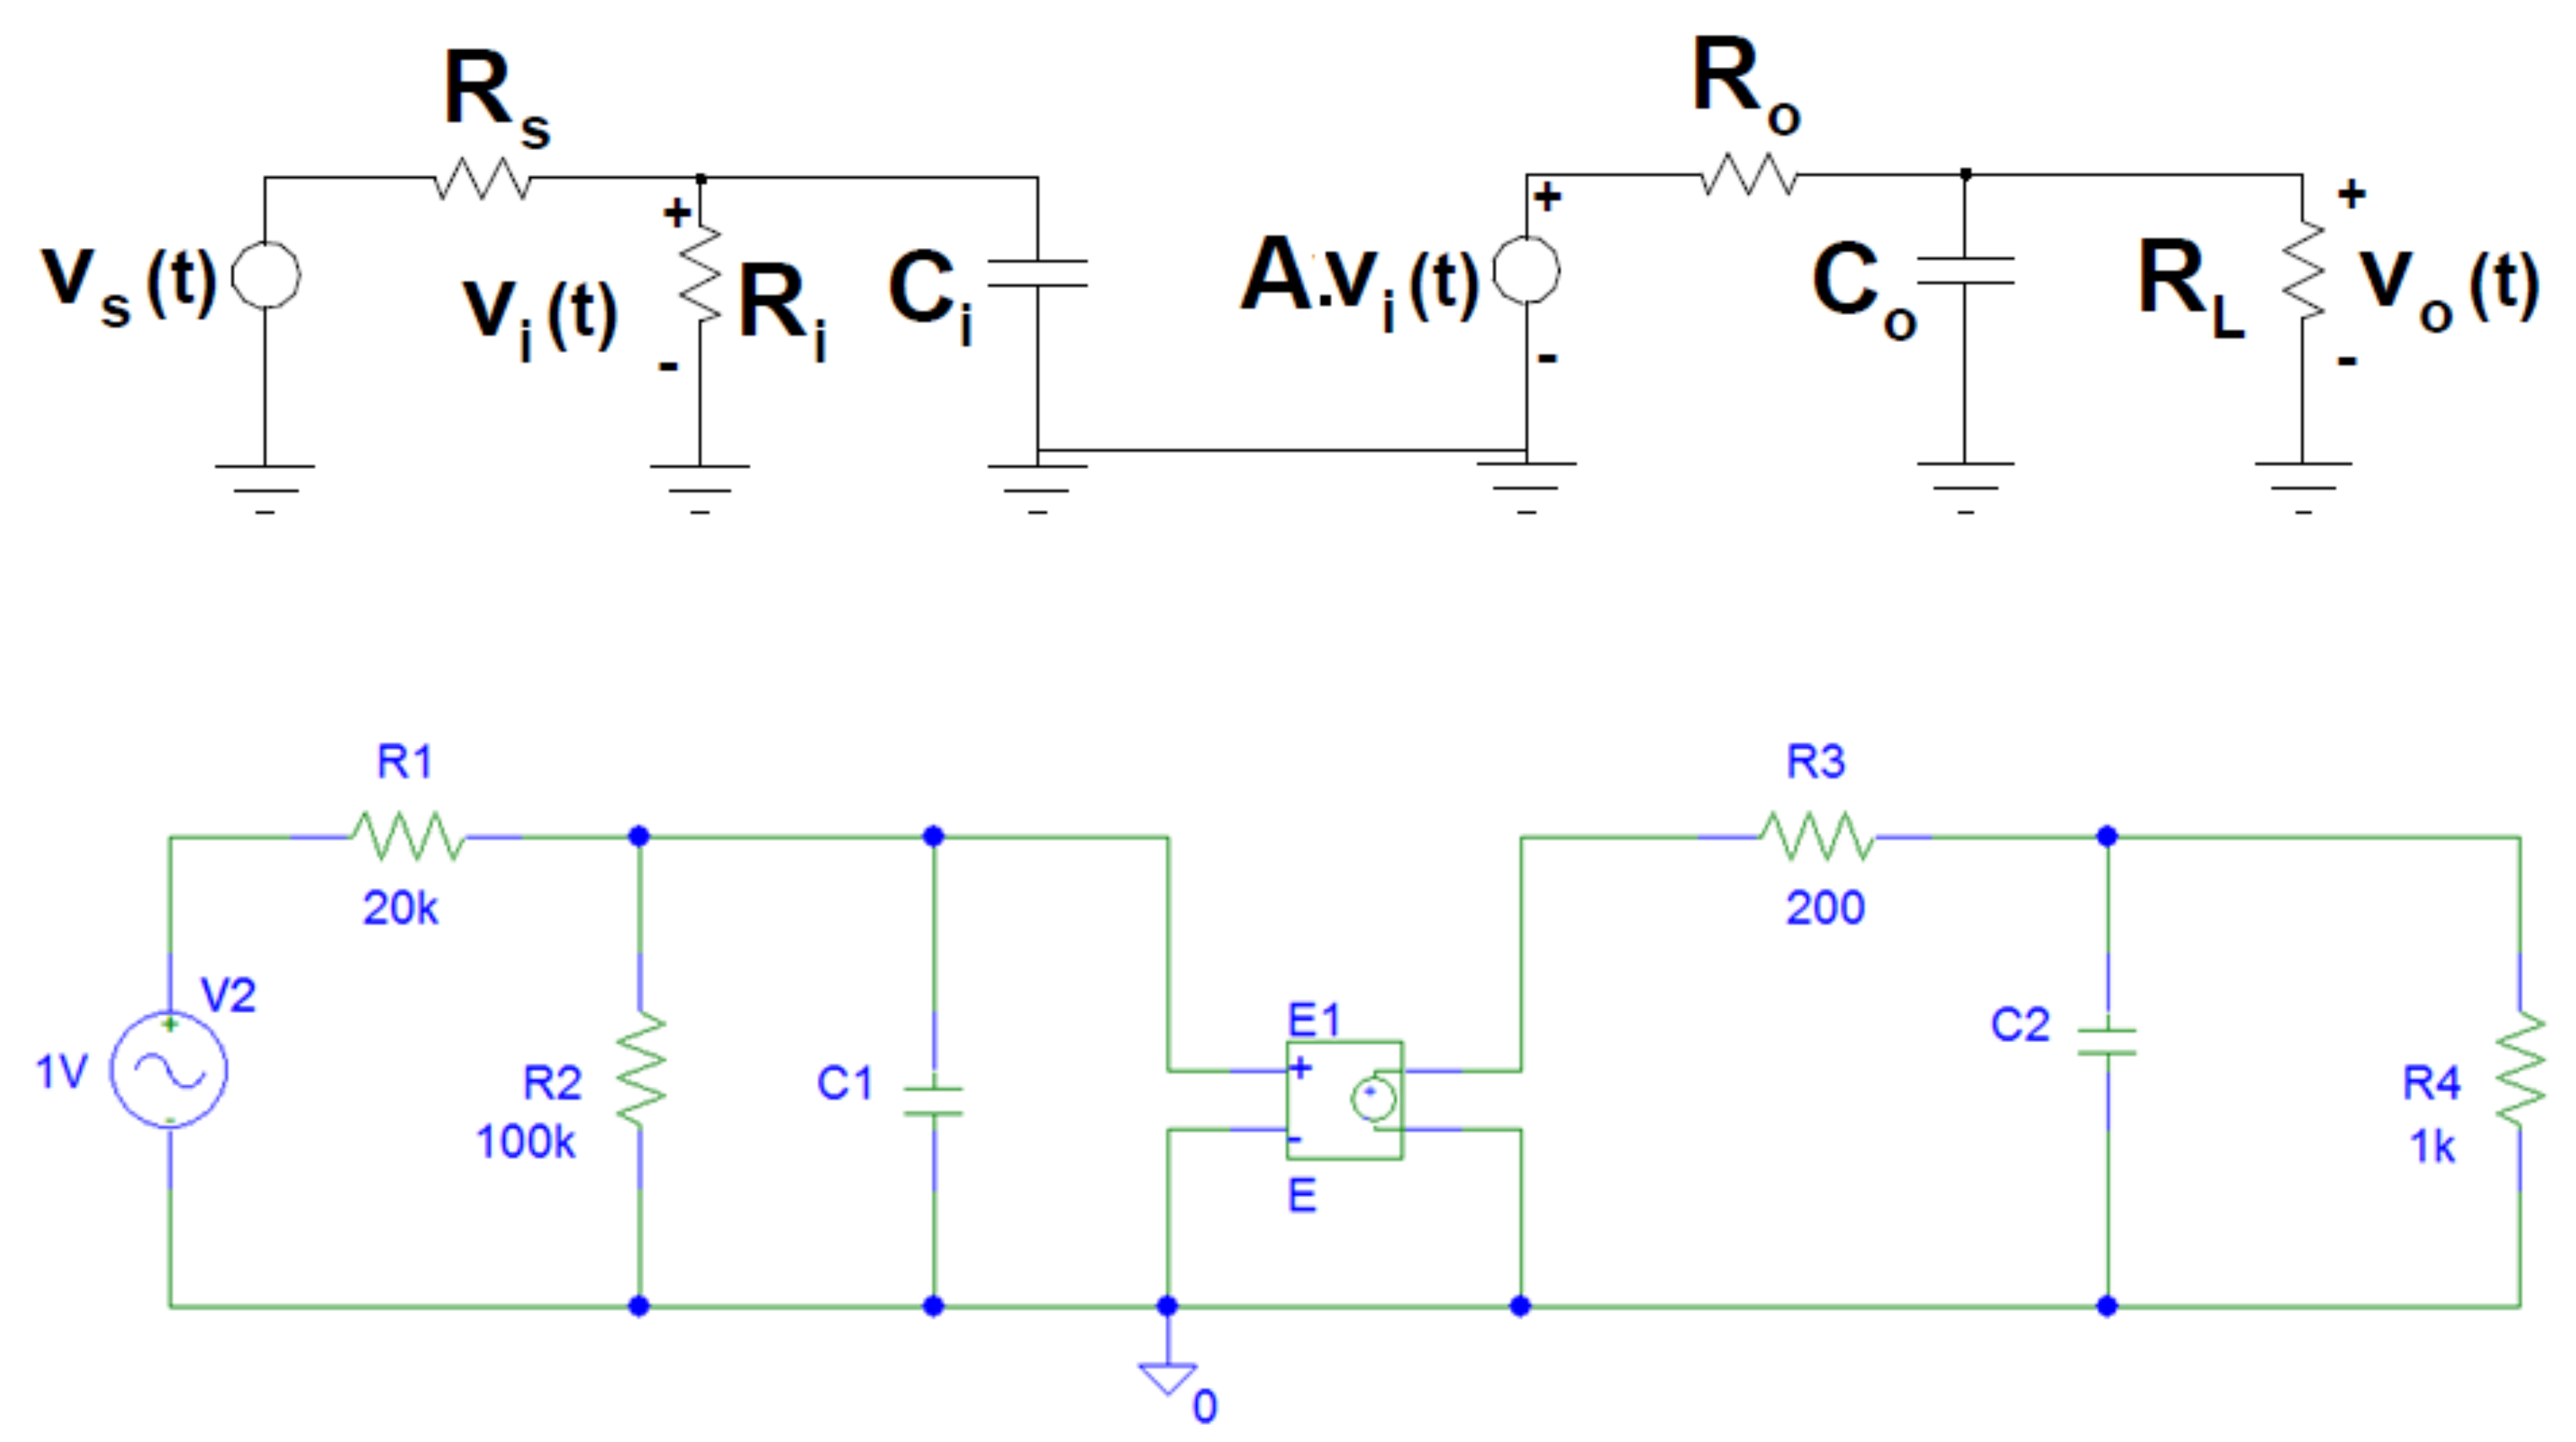
\includegraphics[width=0.9\textwidth]{imagens/1.png}
\end{center}

\question[4] Determine a função de transferência e as constantes de tempo do amplificador porta comum da Figura. \underline{Usando o modelo de pequenos sinais do amplificador}, obtenha o gráfico do módulo da resposta em frequência e fase do amplificador e indique as frequências de corte. Considere:

\begin{minipage}[m]{0.3\textwidth}
\begin{itemize}
    \item $\lambda = 0$
    \item $R_D = 10$ $k\Omega$
    \item $R_S = 5$ $k\Omega$
    \item $C_{IN} = 25$ pF
    \item $C_L = 80$ pF
    \item $W/L = 60+e$
    \item $k'_n = 100$ $\mu A/V^2$
    \item $V_{OV} = 0,8$ V
\end{itemize}
\end{minipage}
\hspace{5mm}
\begin{minipage}[m]{0.4\textwidth}
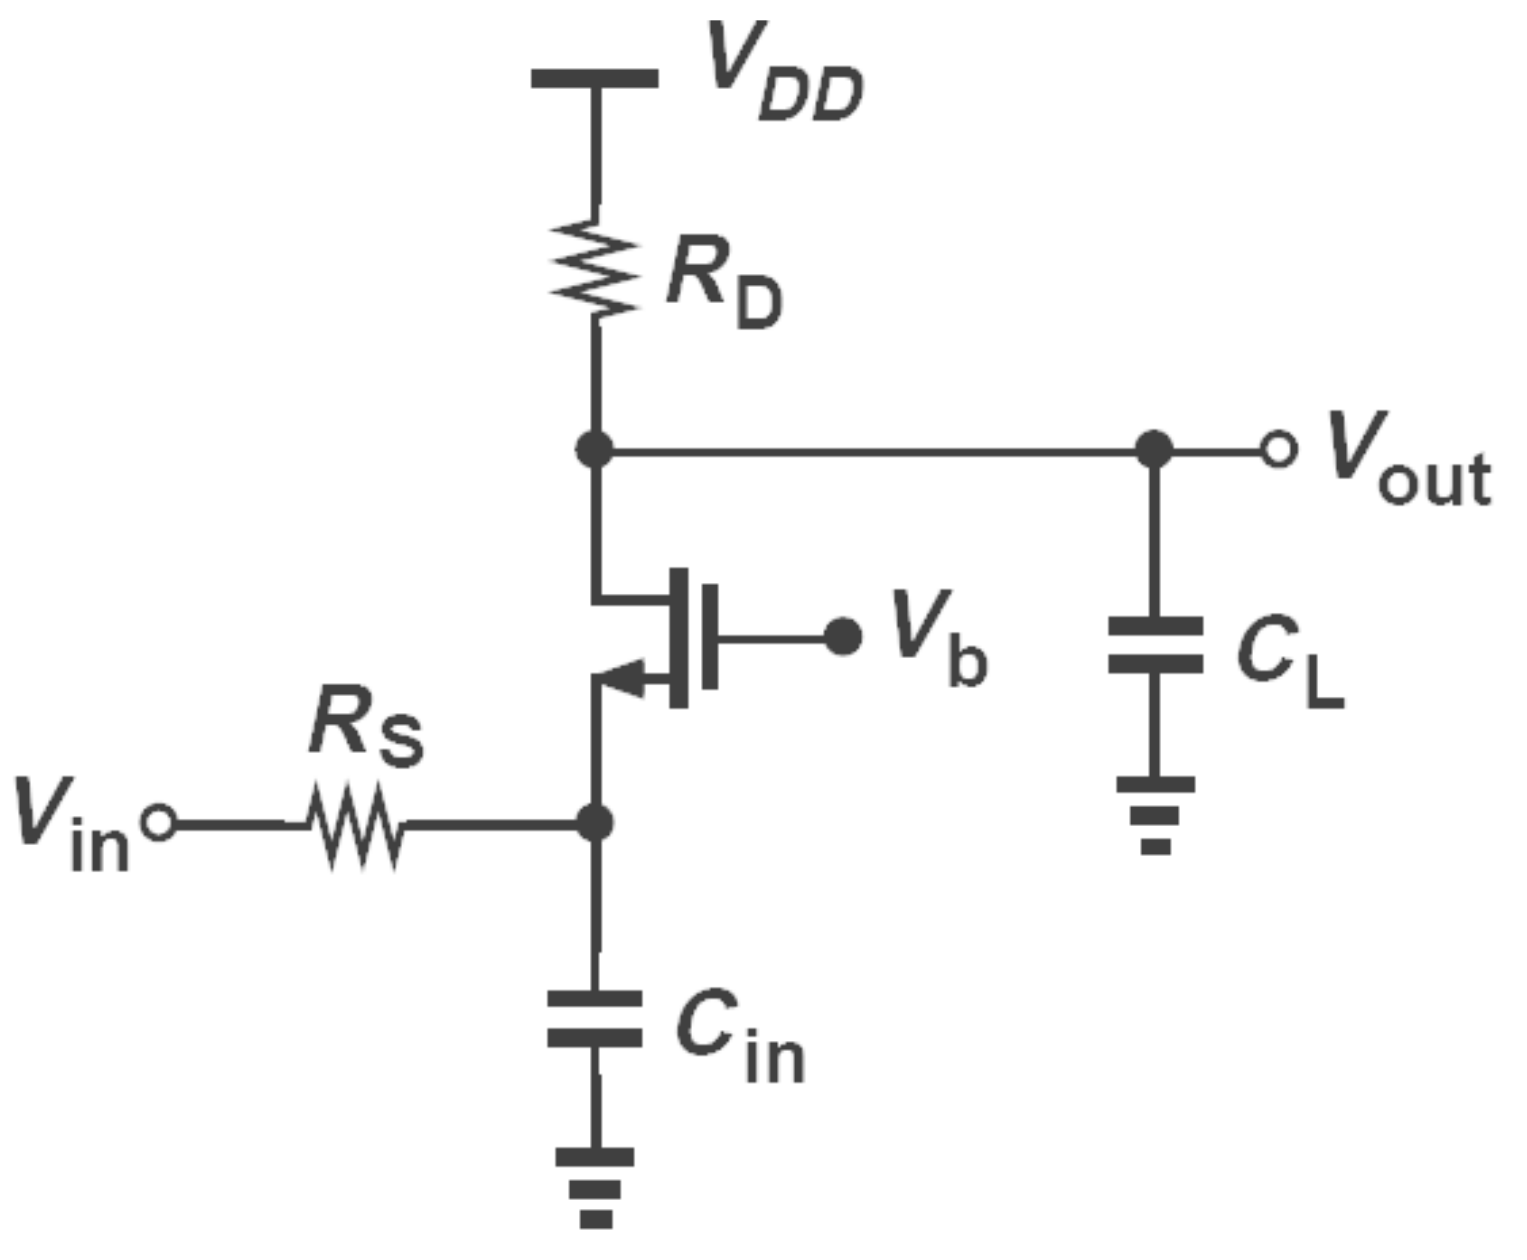
\includegraphics[width=\textwidth]{imagens/2.png}
\end{minipage}

\question[2] Usando o circuito da Figura, levante as curvas necessárias para obter o ganho máximo e a resposta em frequência na faixa de 0,1 Hz a 1000 MHz. O valor de $R_D$ deve ser usado como (10+\textit{\textbf{f}}) $k\Omega$.

\begin{parts}
\part[2] Quais os valores das tensões de $V_{GS}$ e $V_{DS}$? O transistor está na saturação?
\part[1] Quais as frequências de corte superior e inferior do circuito?
\part[1] Qual o consumo total de potência do circuito?
\part[1] Qual o ganho máximo obtido?
\end{parts}

\textbf{Atenção:} Usar o modelo abaixo para o transistor NMOS (Modelo do transistor disponível no Moodle)

.model NMOS0P5 NMOS (level=1 gamma=0.5 tox=9.5n uo=460 phi=0.8 kp=170.1u w=23.3u l=0.44u vto=0.7 pb=0.9 mj=0.5 cgso=0.4n cgdo=0.4n cgbo=0.38u ld=0.08u js=10u cj=0.57m mj=0.5 cjsw=0.12u mjsw=0.4)

\begin{center}
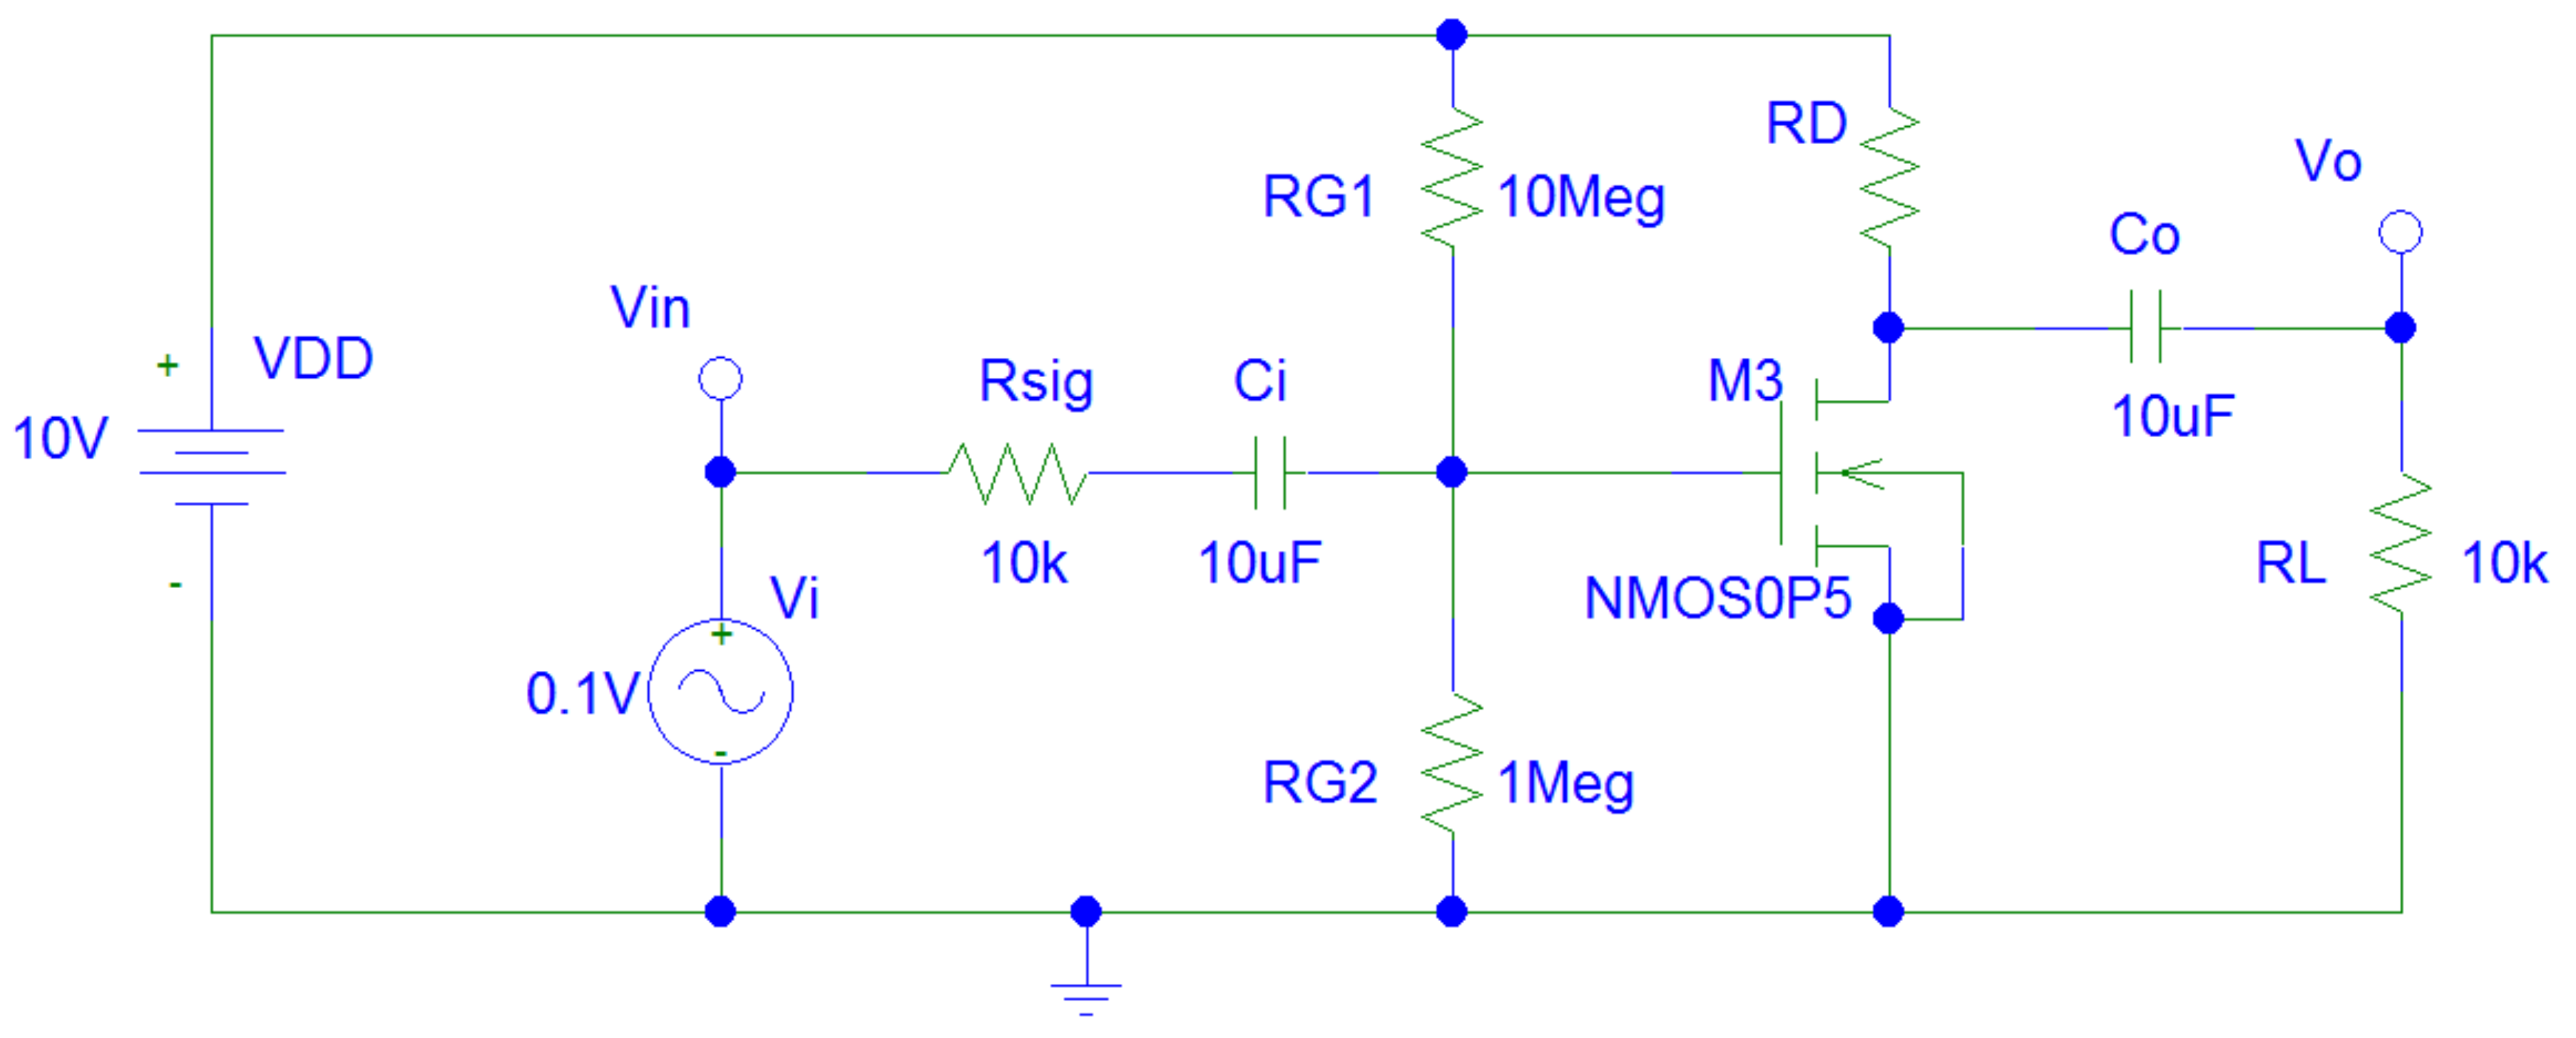
\includegraphics[width=0.9\textwidth]{imagens/3.png} 
\end{center}

\vspace{5mm}

\textbf{REFERÊNCIAS}

\vspace{5mm}

MANERA, Leandro T. \textbf{Vídeos sobre SPICE}. \url{http://www.dsif.fee.unicamp.br/~manera/EE640/download.html}. Acesso em 08-01-2019.

UNIVERSITY OF PENNSYLVANIA. \textbf{Spice model parameters of mosfets}. \url{https://www.seas.upenn.edu/~jan/spice/spice.MOSparamlist.html}. Acesso em 08-01-2019.

\end{questions}

\end{document}
